\chapter{\huge Integrazione Numerica}

\textit{In analisi numerica, l'integrazione numerica consiste in un insieme di metodi che stimano il valore di un integrale definito, senza dover calcolare la primitiva della funzione integranda. In questa sezione si illustrano alcuni dei principali metodi deterministici e non deterministici.}

\section{Newton-Cotes}
Le regole di quadratura di Newton-Cotes sono formule che consistono nel valutare l'integrando in punti equispaziati dell'intervallo di integrazione.

Si assume che il valore di una funzione $f:[a,b]\subset\mathbb{R}\rightarrow\mathbb{R}$ sia noto nei punti $x_i$, per $i=0,...,n$ tali che $$x_i=a+\left(\frac{b-a}{n}\right)i$$
La formula di Newton-Cotes di grado $n$ si ottiene interpolando $f$ nei punti $x_i$ con i polinomi della base di Lagrange~\cite{uno}, e integrando la polinomiale risultante, $L(x)$, nell'intervallo $[a,b]$.
$$ \int_a^b f(x) \,dx \approx \int_a^b L(x)\,dx = \int_a^b \bigl( \sum_{i=0}^n f(x_i)\, \ell_i(x) \bigr) \, dx = \sum_{i=0}^n f(x_i) \underbrace{\int_a^b \ell_i(x)\, dx}_{w_i} $$
dove gli $\ell_i(x)$ sono i polinomi di Lagrange così definiti
$$\ell_i(x):= \prod_{\begin{smallmatrix}0\le j\le n\\ j\neq i\end{smallmatrix}} \frac{x-x_j}{x_i-x_j}$$$$\ell_i(x_j)=\delta_{ij}$$
La formula di Newton-Cotes assume così la semplice forma di media dei valori $f(x_i)$ pesati sui coefficienti $w_i$ (indipendenti da $f$)
$$\int_a^b f(x) \,dx \approx \sum_{i=0}^n w_i\, f(x_i)$$
Si domostra che l'errore dell'interpolazione di $f$ con un polinomio è
$$E(x)=\frac{1}{(n+1)!}f^{(n+1)}(\xi(x))\prod_{i=0}^n(x-x_i)$$
per un certo $\xi\in[a,b]$ dipendente da $x$. Non avendo tuttavia alcuna informazione su come individuare il punto $\xi$ in genere si effettua solo una stima del limite superiore sull'errore $E(x)$ per $\xi$ tale che $f(\xi) = \underset{x\in[a,b]}{\max}f(x)$.

Al primo ordine dell'approssimazione Newton-Cotes la formula si riduce al cosidetto metodo dei ``trapezi'':
$$\int_a^b f(x) \,dx=\frac{b-a}{2}\left[ f(a)+f(b)\right] + \underbrace{\frac{1}{2}\int_a^b f''(\xi(x))(x-a)(x-b)}_{E_1}$$
mentre al secondo ordine non è altro che la regola di Simpson:
\begin{multline*}
\int_a^b f(x) \,dx=\frac{b-a}{3}\left[f(a)+4f(\frac{a+b}{2})+f(b)\right] +\\ + \underbrace{\frac{1}{6}\int_a^b f'''(\xi(x))(x-a)(x-\frac{a+b}{2})(x-b)}_{E_2}
\end{multline*}

\section{Quadrature Gaussiane}
La regola di quadratura Gaussiana a $n$-punti è un metodo di integrazione numerica costruito in modo tale da fornire un risultato esatto per polinomi di grado inferiore a $2n$, attraverso una scelta appropriata di punti $x_i$ e pesi $w_i$, per $i=1,...,n$. Sul dominio di integrazione convenzionale $[-1,1]$ la regola è così formulata
$$\int_{-1}^1 f(x)\,dx \approx \sum_{i=1}^n w_i f(x_i)$$
L'accuratezza del risultato è tanto più grande quanto meglio $f$ è approssimata da un polinomio. Se tuttavia la funzione integranda può essere scritta come $f(x)=W(x)g(x)$, dove $g(x)$ è approssimativamente polinomiale e $W(x)$ è nota, allora esistono $w'_i$ tali che
$$\int_{-1}^1 f(x)\,dx = \int_{-1}^1 W(x) g(x)\,dx \approx \sum_{i=1}^n w_i' g(x_i)$$
$W(x)$ viene detta funzione peso, mentre i punti $x_i$ sono le radici di un polinomio appartenente alla classe dei polinomi ortogonali.

Nel caso considerato $W(x)=1$ ed i polinomi associati sono i polinomi ortogonali di Legendre $P_n(x)$~\cite{uno}. Il peso $i$-esimo associato al nodo Gaussiano $x_i$ è dato da
$$ w_i = \frac{2}{\left( 1-x_i^2 \right) [P'_n(x_i)]^2} \,\!$$
Analogamente alle regole di Newton-Cotes, l'errore teorico del metodo della quadratura Gaussiana è
$$E(x)=\frac{1}{n!}f^{(n)}(\xi(x))\prod_{i=1}^n(x-x_i)$$
che può tuttavia essere ridotto a
$$E(x)=\frac{1}{(2n)!}f^{(2n)}(\xi(x))\prod_{i=1}^n(x-x_i)^2$$
semplicemente considerando due volte ogni punto di interpolazione $x_i$.

Infine, se si vuole calcolare l'integrale su $[a,b]$ invece che sull'intervallo $[-1,1]$, si deve effettuare il cambio di variabile
$$\int_a^b f(x)\,dx = \frac{b-a}{2} \int_{-1}^1 f\left(\frac{b-a}{2}x + \frac{a+b}{2}\right)\,dx $$
ed applicando il metodo di Gauss si ottiene
$$\int_a^b f(x)\,dx \approx \frac{b-a}{2} \sum_{i=1}^n w_i f\left(\frac{b-a}{2}x_i + \frac{a+b}{2}\right)$$
I nodi ed i pesi per il polinomio di Legendre di quinto grado sono riportati in tabella:\\
\begin{center}
\scalebox{1.5}{
\begin{tabular}{c c}
\hline
$x_i$ & $w_i$ \\
\hline\hline
$0$ & $\frac{128}{255}$ \\
$\pm\tfrac13\sqrt{5-2\sqrt{10/7}}$ & $\tfrac{322+13\sqrt{70}}{900}$ \\
$\pm\tfrac13\sqrt{5+2\sqrt{10/7}}$ & $\tfrac{322-13\sqrt{70}}{900}$ \\
\end{tabular}
}
\end{center}

\subsection{Integrazione Composta}
Una tecnica utile a migliorare la precisione del calcolo dell'integrale numerico consiste nello spezzare l'intervallo d'integrazione in $n$ sottointervalli
$$\int_a^b f(x)dx=\sum_{i=0}^{n-1}\int_{\frac{b-a}{n}i}^{\frac{b-a}{n}(i+1)}f(x)dx$$
Dopodiché si applica uno dei metodi di quadratura numerica descritto ad ogni intervallino ed infine si somma ad ottenere il risutato richiesto.

\section{Monte Carlo}
L'integrazione Monte Carlo~\cite{sei}, a differenza dei metodi di quadratura precedentemente descritti, fa uso di sampling casuali e per questo motivo rientra nella categoria dei metodi non deterministici.

Nella sua versione più semplice l'algoritmo consiste nell'estrarre uniformemente punti dalla regione di integrazione per stimare l'integrale ed il relativo errore. Si supponga che il sample sia costituito da $N$ punti $x_1,...,x_N$ appartenenti alla regione di integrazione di misura $V$, allora la stima dell'integrale è data da
$$ I \approx E_N \equiv V\frac{1}{N} \sum_{i=1}^N f(x_i) = V \langle f \rangle $$
Poichè $\{x_i\}$ è una sequenza di punti equidistribuiti in $V$, si può dimostrare che $ I = \lim_{N \to \infty} E_N $.
Tenendo presente che la varianza della funzione integranda è
$$ \mathrm{Var}(f)\equiv\sigma_N^2 = \frac{1}{N-1} \sum_{i=1}^N (f(x_i) - \langle f \rangle)^2$$
la varianza di $E_N$ è quindi
$$ \mathrm{Var}(E_N) =  \frac{V^2}{N^2} \sum_{i=1}^N \mathrm{Var}(f)  =V^2 \frac{\mathrm{Var}(f)}{N} = V^2\frac{\sigma_N^2}{N}$$
Dal momento che le considerazioni appena fatte rimangono valide anche nel caso multidimensionale, quello che si deduce è che l'errore sulla stima dell'integrale scala come $1/\sqrt{N}$, indipendentemente dal numero di dimensioni.

\subsection{Campionamento di Importanza}
Dal punto di vista metematico, il campionamento di importanza corrisponde al cambio di variabile
$$\int f(x) \,dx = \int\frac{f(x)}{p(x)}\,p(x)\,dx = \int\frac{f(x)}{p(x)}\,dP(x)$$
con $$p(x)=\frac{\partial^d}{\partial x_1...\partial x_d}\,P(x)$$
Se si restringe $p(x)$ ad essere una funzione a valori non negativi normalizzata all'unità, allora si può interpretare $p(x)$ come una densità di probabilità. Se poi si ha a disposizione un generatore di numeri casuali corrispondente alla distribuzione $P(x)$ si può anche stimare l'integrale da un sample $x_1,...,x_N$ di numeri casuali distribuiti secondo $P(x)$
$$E_N = \frac{1}{N}\sum_{n=1}^N\frac{f(x_n)}{p(x_n)}$$
L'errore statistico dell'integrazione Monte Carlo è dato da $\sigma(f/p)/\sqrt N$.

Il campionamento di importanza è efficace se si sceglie $p(x)$ tale che approssimi bene $|f(x)|$ e tale che si sia capaci di generare numeri casuali con distribuzione di probabilità $P(x)$.

\section{Esempi}
Si dimostrano ora i metodi descritti nei paragrafi precedenti applicandoli al calcolo di alcuni integrali particolari. Le funzioni integrande scelte sono:
\begin{figure}[H]
\centering
\begin{tabular}{lccl}
funzione & & & primitiva\\\\
$\log(1+x)$ & & & $-x + \log(1 + x) + x \log(1 + x)$\\\\
$x^9 - x^7 + 3$ & & & $\frac{x^{10}}{10} - \frac{x^8}{8} + 3x$
\end{tabular}
\end{figure}
Tutti gli integrali sono calcolati tenendo fisso l'intervallo d'integrazione $I=[1,2]$ e variando il numero di suddivisioni per ogni metodo. Conoscendo inoltre l'espressione analitica delle primitive delle due funzioni integrande è possibile calcolare i risultati esatti ed usare questi ultimi per confrontare l'errore del risultato numerico con l'errore previsto. Si sono calcolati analiticamente dunque alcuni valori utili alla stima di tale errore:
\\

\begin{figure}[H]
\centering
\begin{tabular}{ccc}
$f$ & $\max(f^{(1)})$ & $\max(f^{(4)})$\\
\hline
$\log(1+x)$ & $0.5$ & $-0.0740742$\\
$x^9 - x^7 + 3$ & $1856$ & $90048$
\end{tabular}
\end{figure}

In seguito si indicheranno con $E(f)$ l'errore stimato analiticamente e con $\Delta(f)$ l'errore calcolato numericamente.

\subsection{Newton-Cotes 1}

\begin{figure}[H]
 \begin{subfigure}[b]{0.5\textwidth}
  \centering
  \includegraphics[width=\textwidth]{integral1a}
  \caption{Log}
 \end{subfigure}
 \begin{subfigure}[b]{0.5\textwidth}
  \centering
  \includegraphics[width=\textwidth]{integral1b}
  \caption{Pol}
 \end{subfigure}
\caption{Confronto errore NC1 calcolato numericamente (rosso) e previsto analiticamente (blu).}
\label{fig:integral1}
\end{figure}

\begin{figure}[H]
 \begin{subtable}[b]{0.5\textwidth}
  \centering\small
\begin{tabular}{lll}
\hline
$n$ & $\Delta(Log)$ & $E(Log)$\\
\hline
10 & 1.388645e-04 & 4.166667e-04\\
20 & 3.472070e-05 & 1.041667e-04\\
40 & 8.680460e-06 & 2.604167e-05\\
80 & 2.170133e-06 & 6.510417e-06\\
160 & 5.425343e-07 & 1.627604e-06\\
320 & 1.356337e-07 & 4.069010e-07\\
640 & 3.390842e-08 & 1.017253e-07\\
1280 & 8.477104e-09 & 2.543132e-08\\
2560 & 2.119278e-09 & 6.357829e-09\\
5120 & 5.298190e-10 & 1.589457e-09\\
10240 & 1.324540e-10 & 3.973643e-10\\
20480 & 3.311029e-11 & 9.934107e-11\\
40960 & 8.277934e-12 & 2.483527e-11\\
81920 & 2.073119e-12 & 6.208817e-12\\
\end{tabular}
 \end{subtable}
 \begin{subtable}[b]{0.5\textwidth}
  \centering\small
\begin{tabular}{lll}
\hline
$n$ & $\Delta(Pol)$ & $E(Pol)$\\
\hline
10 & 1.541035e+00 & 1.546667e+00\\
20 & 3.860018e-01 & 3.866667e-01\\
40 & 9.654698e-02 & 9.666667e-02\\
80 & 2.413966e-02 & 2.416667e-02\\
160 & 6.035096e-03 & 6.041667e-03\\
320 & 1.508785e-03 & 1.510417e-03\\
640 & 3.771970e-04 & 3.776042e-04\\
1280 & 9.429930e-05 & 9.440104e-05\\
2560 & 2.357483e-05 & 2.360026e-05\\
5120 & 5.893707e-06 & 5.900065e-06\\
10240 & 1.473427e-06 & 1.475016e-06\\
20480 & 3.683568e-07 & 3.687541e-07\\
40960 & 9.208927e-08 & 9.218852e-08\\
81920 & 2.302198e-08 & 2.304713e-08\\
\end{tabular}
 \end{subtable}
\end{figure}

Come previsto, l'errore calcolato segue l'andamento ricavato analiticamente pur rimanendo sempre al di sotto di quest'ultimo. $E(f)$ infatti è solo il limite superiore per l'errore $\Delta(f).$ Nel caso della polinomiale inoltre i due errori risultano particolarmente vicini.

\subsection{Newton-Cotes 2}

\begin{figure}[H]
 \begin{subfigure}[b]{0.5\textwidth}
  \centering
  \includegraphics[width=\textwidth]{integral2a}
  \caption{Log}
 \end{subfigure}
 \begin{subfigure}[b]{0.5\textwidth}
  \centering
  \includegraphics[width=\textwidth]{integral2b}
  \caption{Pol}
 \end{subfigure}
\caption{Confronto errore NC2 calcolato numericamente (rosso) e previsto analiticamente (blu).}
\label{fig:integral2}
\end{figure}

\begin{figure}[H]
 \begin{subtable}[b]{0.5\textwidth}
  \centering\small
\begin{tabular}{lll}
\hline
$n$ & $\Delta(Log)$ & $E(Log)$\\
\hline
10 & 6.101824e-09 & 8.230467e-08\\
20 & 3.816787e-10 & 5.144042e-09\\
40 & 2.386025e-11 & 3.215026e-10\\
80 & 1.491696e-12 & 2.009391e-11\\
160 & 9.325873e-14 & 1.255870e-12\\
320 & 6.328271e-15 & 7.849185e-14\\
640 & 5.551115e-16 & 4.905740e-15\\
1280 & 1.443290e-15 & 3.066088e-16\\
2560 & 1.110223e-15 & 1.916305e-17\\
5120 & 2.442491e-15 & 1.197691e-18\\
10240 & 1.443290e-15 & 7.485566e-20\\
20480 & 4.440892e-15 & 4.678479e-21\\
40960 & 9.992007e-16 & 2.924049e-22\\
81920 & 3.996803e-15 & 1.827531e-23\\
\end{tabular}
 \end{subtable}
 \begin{subtable}[b]{0.5\textwidth}
  \centering\small
\begin{tabular}{lll}
\hline
$n$ & $\Delta(Pol)$ & $E(Pol)$\\
\hline
10 & 9.908609e-04 & 1.000533e-01\\
20 & 6.203492e-05 & 6.253333e-03\\
40 & 3.878841e-06 & 3.908333e-04\\
80 & 2.424535e-07 & 2.442708e-05\\
160 & 1.515373e-08 & 1.526693e-06\\
320 & 9.471108e-10 & 9.541829e-08\\
640 & 5.920242e-11 & 5.963643e-09\\
1280 & 3.666401e-12 & 3.727277e-10\\
2560 & 1.421085e-13 & 2.329548e-11\\
5120 & 1.278977e-13 & 1.455968e-12\\
10240 & 2.842171e-14 & 9.099798e-14\\
20480 & 4.263256e-14 & 5.687374e-15\\
40960 & 7.105427e-14 & 3.554608e-16\\
81920 & 5.684342e-14 & 2.221630e-17\\
\end{tabular}
 \end{subtable}
\end{figure}

L'errore per il metodo NC2 si comporta come previsto finchè non raggiunge valori dell'ordine di grandezza di $10^{-14}$ per i quali la precisione finita del calcolatore limita la precisione del calcolo introducendo del rumore nei dati.

\subsection{Quadratura Gaussiana 5}

\begin{figure}[H]
 \begin{subtable}[b]{0.5\textwidth}
  \centering
\begin{tabular}{lll}
\hline
$n$ & $\Delta(Log)$\\
\hline
10 & 2.220446e-16\\
20 & 2.220446e-16\\
40 & 1.110223e-16\\
80 & 0.000000e+00\\
160 & 5.551115e-16\\
320 & 1.110223e-15\\
640 & 2.220446e-16\\
1280 & 1.332268e-15\\
2560 & 1.110223e-15\\
5120 & 2.664535e-15\\
10240 & 1.110223e-16\\
20480 & 4.440892e-15\\
40960 & 9.992007e-16\\
81920 & 3.996803e-15\\
\end{tabular}
 \end{subtable}
 \begin{subtable}[b]{0.5\textwidth}
  \centering
\begin{tabular}{lll}
\hline
$n$ & $\Delta(Pol)$\\
\hline
10 & 0.000000e+00\\
20 & 0.000000e+00\\
40 & 0.000000e+00\\
80 & 0.000000e+00\\
160 & 0.000000e+00\\
320 & 1.421085e-14\\
640 & 0.000000e+00\\
1280 & 1.421085e-14\\
2560 & 1.136868e-13\\
5120 & 1.136868e-13\\
10240 & 1.421085e-14\\
20480 & 4.263256e-14\\
40960 & 8.526513e-14\\
81920 & 5.684342e-14\\
\end{tabular}
 \end{subtable}
\end{figure}

Nel caso della quadratura gaussiana di quinto grado l'errore decresce molto più rapidamente, tanto che già con poce decine di intervalli il risultato può essere considerato sufficientemente preciso. Dopo di chè i dati sono troppo disturbati dal rumore per poterne ricavare un andamento funzionale. Si nota inoltre che per il polinomio l'errore è esattamente zero come previsto dalla teoria.
\\

\subsection{Monte Carlo}
\begin{figure}[H]
\begin{subfigure}[b]{0.5\textwidth}
\centering
\includegraphics[width=\textwidth]{integral4a}
\caption{Log}
\end{subfigure}
\begin{subfigure}[b]{0.5\textwidth}
\centering
\includegraphics[width=\textwidth]{integral4b}
\caption{Pol}
\end{subfigure}
\caption{In rosso l'errore MC in funzione del numero di elementi del sample ed in blu la funzione $1/\sqrt{N}$.}
\label{fig:integral4}
\end{figure}

Per analizzare il comportamento dell'errore dei metodi Molte Carlo si studia ora il caso di un integrale di volume bidimensionale. Il dominio di integrazione è l'insieme $\Omega = \{(x,y)\in \mathbb{R}\,|\, x^2+y^2<1\,\wedge\, x,y>0\}$ mentre la funzione integranda non è altro che la costante $1$. Si utilizza la convenzionale funzione di misura $d\mu=dxdy$. La misura di $\Omega$ allora è facile da calcolare essendo l'area di un quarto di circonferenza goniometrica: $$\int_\Omega d\mu = \tfrac{\pi}{4}$$
La distribuzione dell'errore MC in funzione del numero di elementi del sample deve verificare la relazione $\sigma_{MC}\simeq 1/\sqrt N$.
\\

In figura \ref{fig:pi} sono rappresentati in scala bilogaritmica i dati ottenuti da $50000$ esecuzioni dell'algoritmo implementante il metodo Monte Carlo. In ascissa sono riportati i numeri delle dimensioni del sample mentre sulle ordinate sono ripotati i rispettivi errori.\\
Come previsto, la distribuzione ottenuta risulta centrata sulla curva $1/\sqrt{N}$ che è proprio l'errore stimato teoricamente.
\begin{figure}[H]
\centering
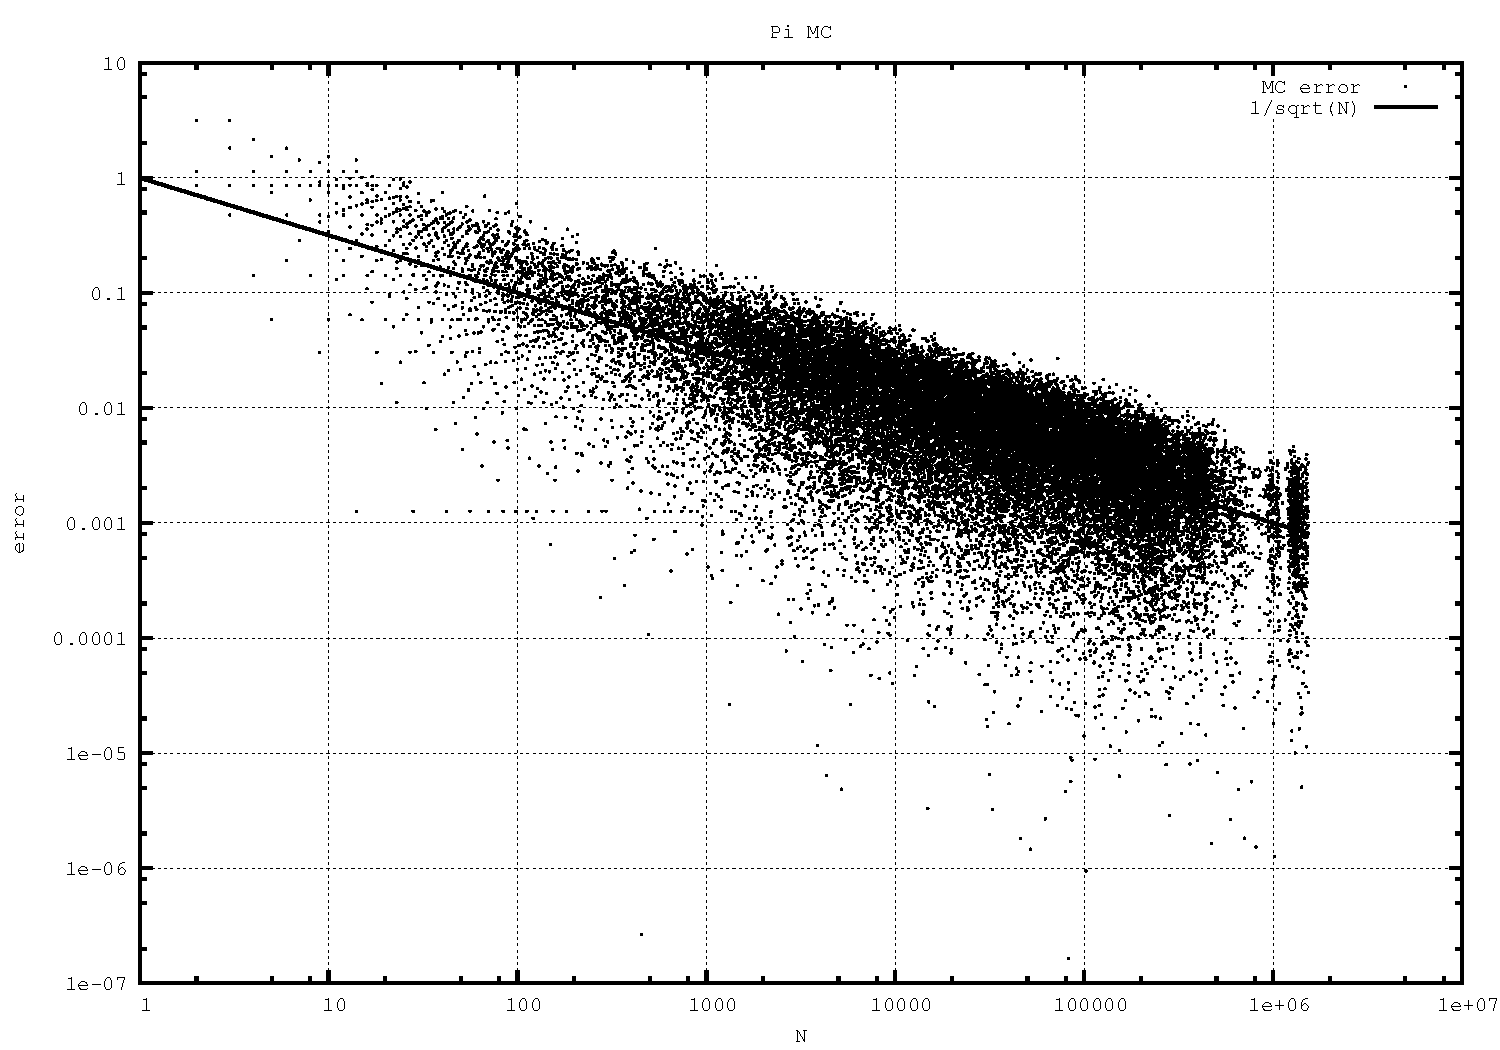
\includegraphics[width=\textwidth]{pi}
\caption{Distribuzione dell'errore MC in funzione del numero di elementi del sample. La linea continua rappresenta la funzione $1/\sqrt{N}$.}
\label{fig:pi}
\end{figure}

